\section{results}
\subsection{Microphone Data}
During the collection process the data from the microphones is actively plotted to ensure the data is being place in the correct frequency bin. 
\begin{figure}[h!]
    \centering
    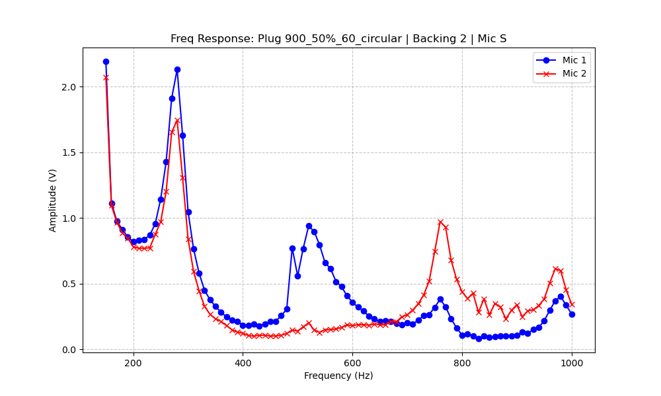
\includegraphics[width=0.7\linewidth]{Microphone_data1.png}
    \caption{Microphone Data with Original Microphone Configuration}
    \label{fig:Mic_data_orig_config}
\end{figure}
Fig \ref{fig:Mic_data_orig_config}. is the data collected with mic 1 on top and mic 2 on bottom. When the microphones have been swapped, the data is again plotted.
\begin{figure}[h!]
    \centering
    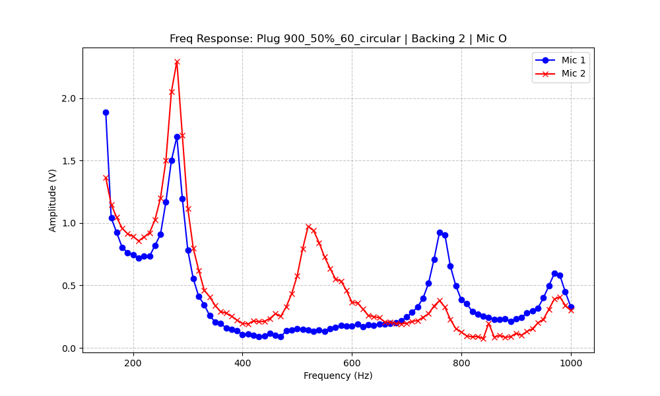
\includegraphics[width=0.7\linewidth]{Microphone_data2.png}
    \caption{Microphone Data with Swapped Microphone Configuration}
    \label{fig:Mic_data_swapped}
\end{figure}
To verify the reproducibility of our data we can compare mic 1 of Fig. \ref{fig:Mic_data_orig_config}
to mic 2 of Fig. \ref{fig:Mic_data_swapped}. These two paths should look similar since they are detecting the pressure at the same location and the same acoustic environment.
\subsection{Intrinsic Properties}
Once the microphone data has been collected. The transfer function can be used to find the values of the propagation constant ($\gamma$) and the characteristic impedance ($Z_c$). Those values are plotted in Fig. \ref{fig:Intrinsic_plot}.

\begin{figure}[h!]
    \centering
    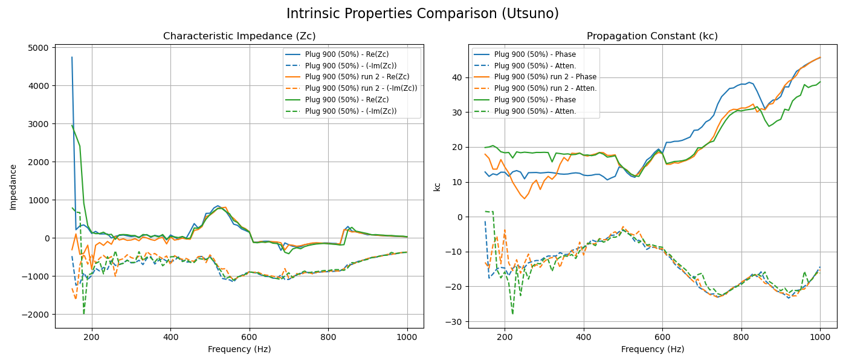
\includegraphics[width=0.8\linewidth]{Intrinsic_properties_graph.png}
    \caption{Intrinsic Properties of 900 60 Millimeter Pores with 50\% Porosity}
    \label{fig:Intrinsic_plot}
\end{figure}
This figure shows the characteristic impedance and propagation constant for a 900 pore 50\% porous medium with 60 mm pores. Three seperate runs are plotted on the same figure. The intrinsic properties are complex numbers, so the imaginary part of each is reflected over the x-axis. This medium interestingly shows a significant increase in acoustic impedance from 500 to 600 Hz. This result was reproducible from run to run. The results from a 20 \% porous medium with 900 pores and a length of 90 millimeter pores were also plotted in Fig. \ref{fig:Intrinsic_plot_2}.

% Figure showing the data from the 90 mm Plug below with label Intrinsic_plot_2
\begin{figure}[h!]
    \centering
    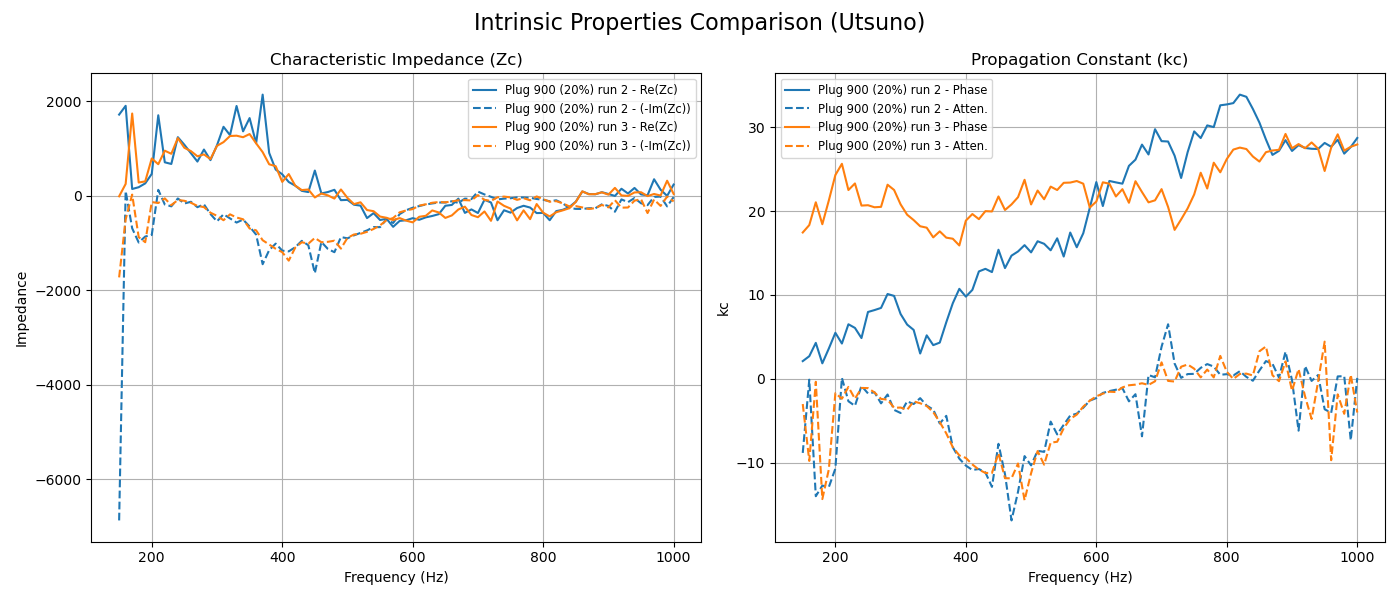
\includegraphics[width=0.8\linewidth]{900-20-90-12bit_combined_graph.png}
    \caption{Intrinsic Properties of 900 90 Millimeter Pores with 20\% Porosity}
    \label{fig:Intrinsic_plot_2}
\end{figure}
This figure shows a noticeable characteristic impedance spike in the lower frequency range. This impedance spike is roughly 300 ($Hz$) lower than Fig. \ref{fig:Intrinsic_plot}. In both figures, the lower frequencies have noticeably more variation in the data. This is attributed to the small surface area of the speaker not being able to push the required volumes of air for lower frequencies.

\subsection{Visualization of intrinsic properties}
The data plotted in Fig. \ref{fig:Intrinsic_plot} and \ref{fig:Intrinsic_plot_2} have been used to create a model that visualizes wave propagation through three distinct regions: incident air, porous sample, and back cavity. The equations outlined in section \ref{sec: Internal Wave Equations} are used to animate the wave in the tube. This visual shows the evolution of the acoustic environment for each individual frequency.

%Add in Animation 1 of the 900 pore 50% porous

Fig. \ref{fig:model_intrinsic_properties} shows the acoustic environment created by the data in Fig. \ref{fig:Intrinsic_plot}. 

\begin{figure}[h!]
    \centering
    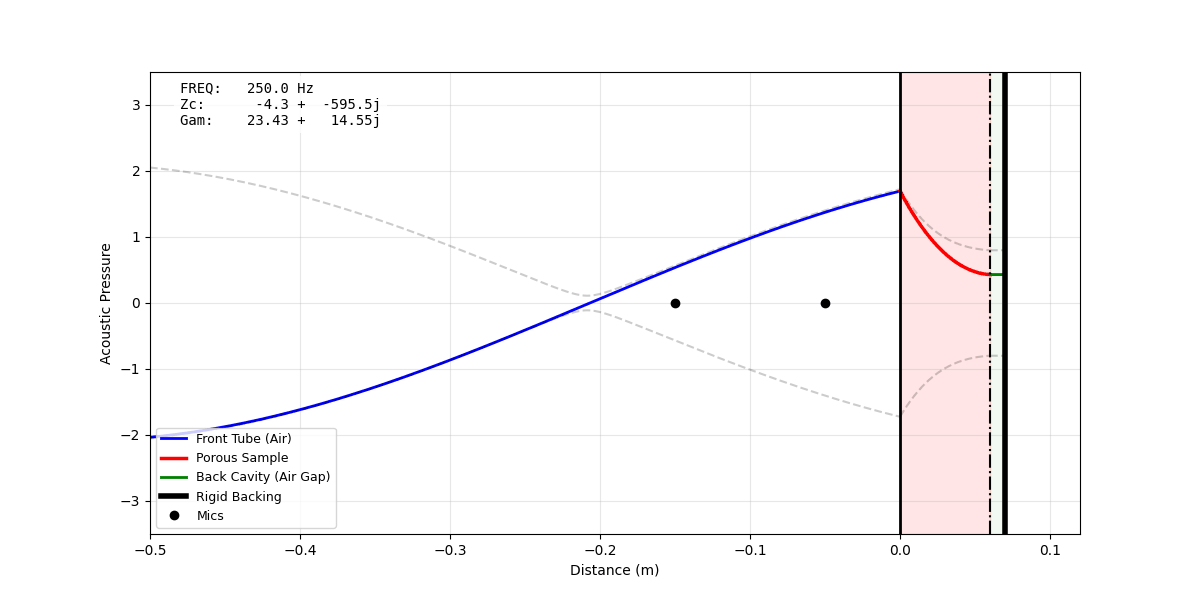
\includegraphics[width=0.7\linewidth]{acoustic_wave_60.png}
    \caption{Intrinsic Properties of the 60 Millimeter 50\% Porosity Medium}
    \label{fig:model_intrinsic_properties}
\end{figure}

Now the data from Fig. \ref{fig:Intrinsic_plot_2} is also shown in Fig. \ref{fig:model_intrinsic_properties_2}.
%Add in animation 2 
\begin{figure}[h!]
    \centering
    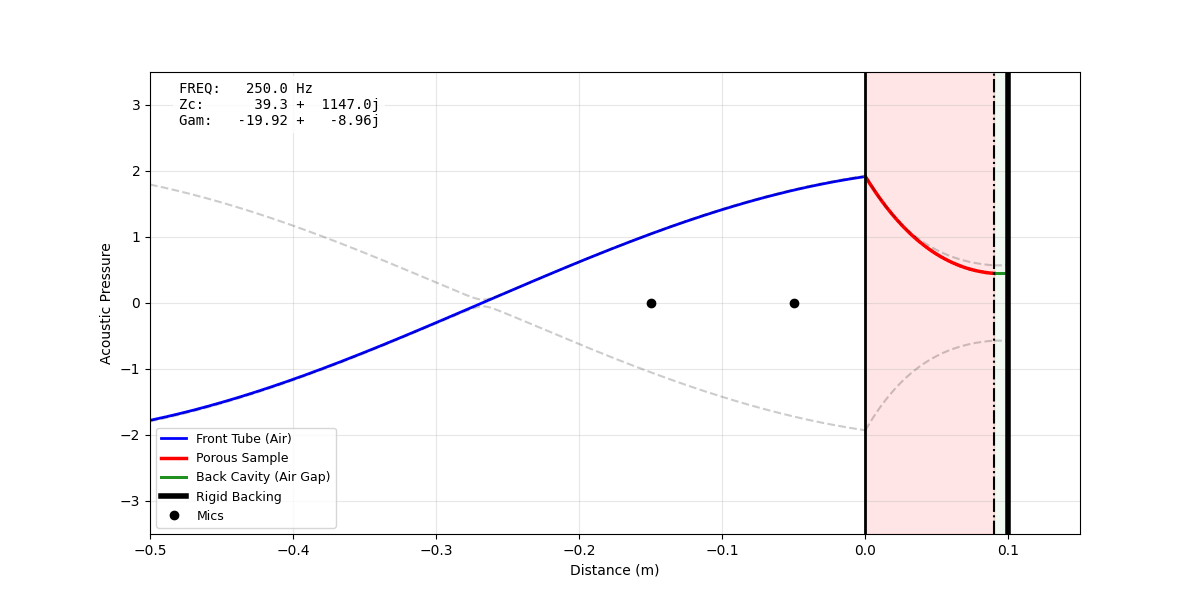
\includegraphics[width=0.7\linewidth]{acoustic_wave_90_20.png}
    \caption{Intrinsic Properties of 90 Millimeter 20\% porous medium modeled}
    \label{fig:model_intrinsic_properties_2}
\end{figure}
These models demonstrate the increased attenuation through the 90 millimeter pug when compared to the 60 millimeter, which is to be expected. This model gives a physical intuition of the experimental data, and allows for the easy identification of non-physical data
%Add in the animation for 900 pores 20% porous 
